

%%%%%%%%%%%%%%%%%%%%%%%%%%%%%%%%%%%%%%%%%%%%%%%%%%%%%%%%%%%%%%%%%%%%%%%%%%%%%%%%%%%%%%%%%%%%%%%%%%%%%%%%%


%
\newpage
\section{Предлагаемая схема информационных потоков в БП}

\subsection{Процессы 'Подготовка производства', 'Учет технологической оснастки'}
%%
\begin{figure}
\begin{center}
  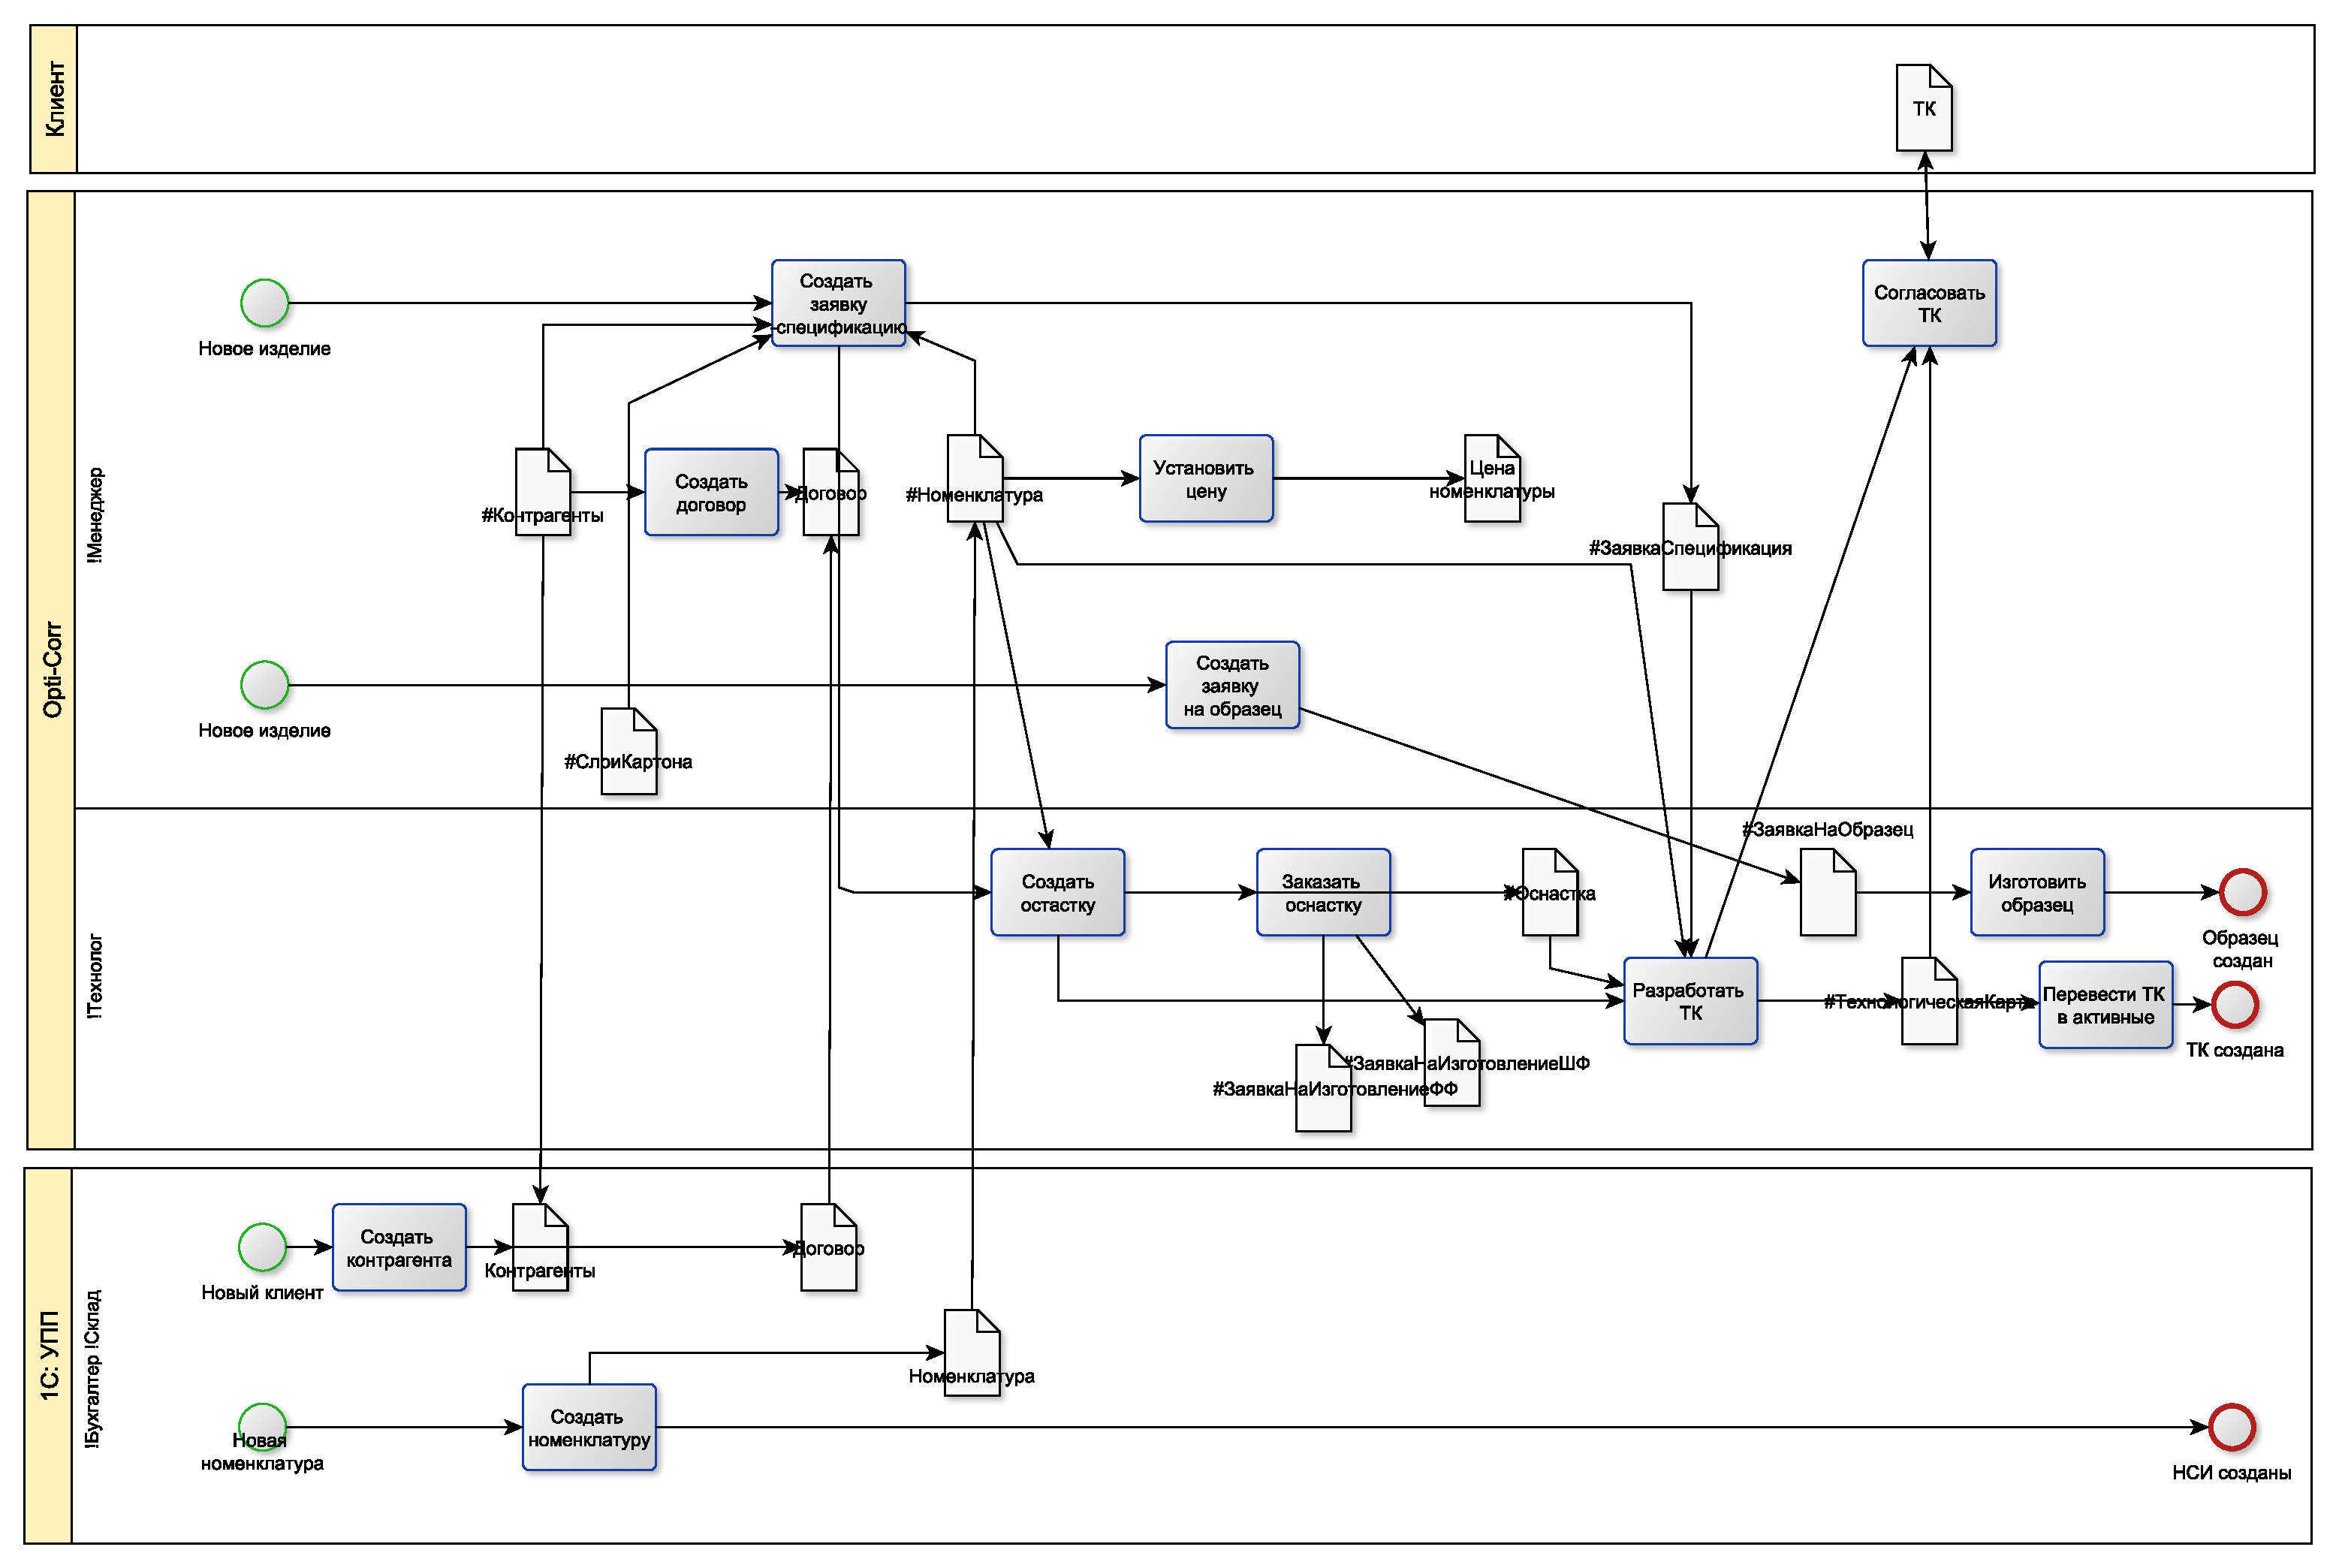
\includegraphics[angle=90, height=0.9\textheight, keepaspectratio]{Pics/1_Новые изделия.pdf}
\end{center}
  \caption{Процессы 'Подготовка производства', 'Учет технологической оснастки'}
  \label{pic:Schema_1}
\end{figure}
\clearpage

При появлении нового контрагента менеджер будет создавать в справочнике ''Контрагенты'' новый элемент справочника в системе Opti-Corrugated для покупателей. В систему 1С:УПП новые элементы будут загружены автоматически.


% При автоматическом обмене СБИС выгрузит новый элемент ''Контрагенты'' в систему  Опти-Софт (СИСТЕМА). При обмене справочники ''Контрагенты'' будут синхронизированы. 

Менеджер при появлении требований от заказчика рассчитывает цену продажи изделия в 1С:УПП. После согласования цены при необходимости менеджер создает автоматически номенклатуру нового изделия в справочнике ''Номенклатура'' в СИСТЕМЕ. 

При автоматическом обмене система 1С:УПП выгрузит новый элемент ''Номенклатура'' в систему Опти-Софт и загрузит новые обратно. При обмене справочники ''Номенклатура'' будут синхронизированы. 

% На основании выполненного расчета цены менеджер формирует печатную форму коммерческого предложения и высылает клиенту. %Есть возможность выслать предложение прямо из СИСТЕМЫ.
% Менеджер будет формировать печатную форму договора и спецификации цены из системы 1С:УНФ. 

После согласования цены менеджер создает в СИСТЕМЕ документ ''Заявка-спецификация'' -- распоряжение технологу по разработке оснастки и технологической карты. 

Отдел главного технолога создает технологическую карту в СИСТЕМЕ, которую менеджер должен согласовать в печатном виде с заказчиком. 



\subsection{Процессы ''Управление продажами''}
%%
\begin{figure}
\begin{center}
  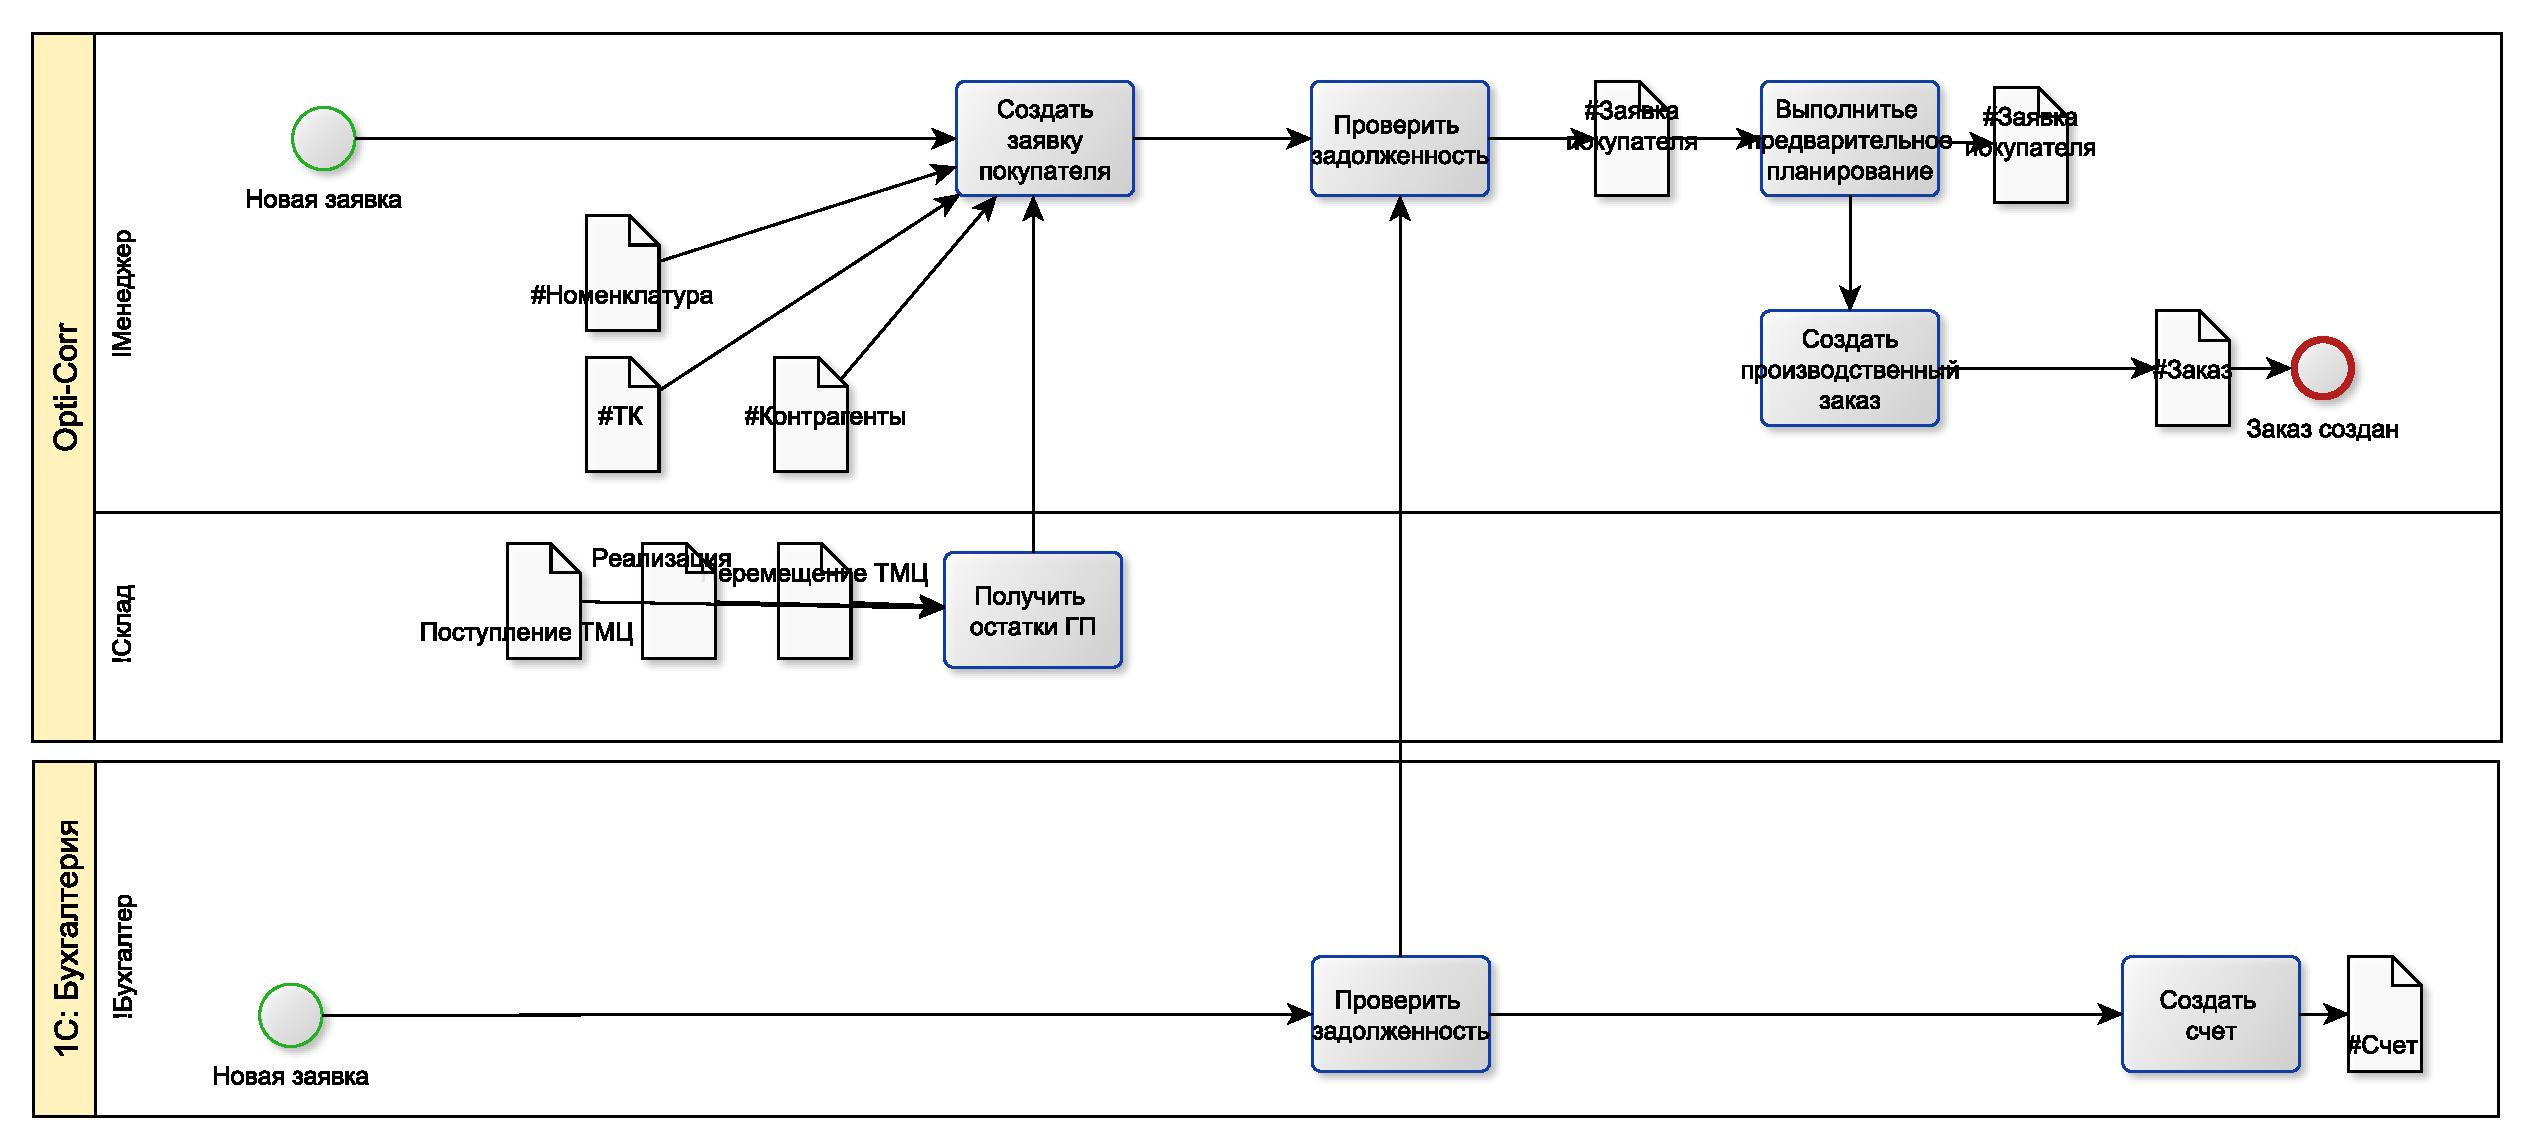
\includegraphics[angle=90, height=0.9\textheight, keepaspectratio]{Pics/2_Продажи.pdf}
\end{center}
  \caption{Процессы ''Управление продажами''}
  \label{pic:Schema_2}
\end{figure}
\clearpage
% %
% Модуль CRM будет работать в системе 1С:УНФ.




После согласования технологической карты менеджер может создать в СИСТЕМЕ заявку покупателя. При создании заявки покупателя СИСТЕМА проверяет остатки по готовой продукции на складе по данным учета системы 1С:УПП. Остатки будут выгружаться из системы 1С:УПП автоматически на утро каждого дня. Текущие остатки по готовой продукции можно будет проверить по данным системы 1С:УПП.

% %, автоматически проверяет задолженность по покупателю на основе данных программы 1С: Бухгалтерия. 

% %В документе ''Заявка'' менеджер должен выбрать организацию внутреннюю. 
% %Менеджер при необходимости будет выполнять расчет предварительной загрузки транспорта.


Менеджер выполняет в СИСТЕМЕ предварительное планирование, при котором СИСТЕМА подскажет возможную дату выполнения производственного заказа. 
Менеджер  утверждает плановую дату производства для позиций заявки.

После согласования условий с клиентом для запуска заявки в производство менеджер должен поменять статус заявки на "Одобрено к выпуску". После согласования даты менеджер создает производственный заказ. После изменения статуса заказы видны в СИСТЕМЕ у планировщика. 
   
% %\newpage
% %%
\subsection{Процессы 'Предварительное планирование', 'Оперативное планирование'}
%
\begin{figure}
\begin{center}
  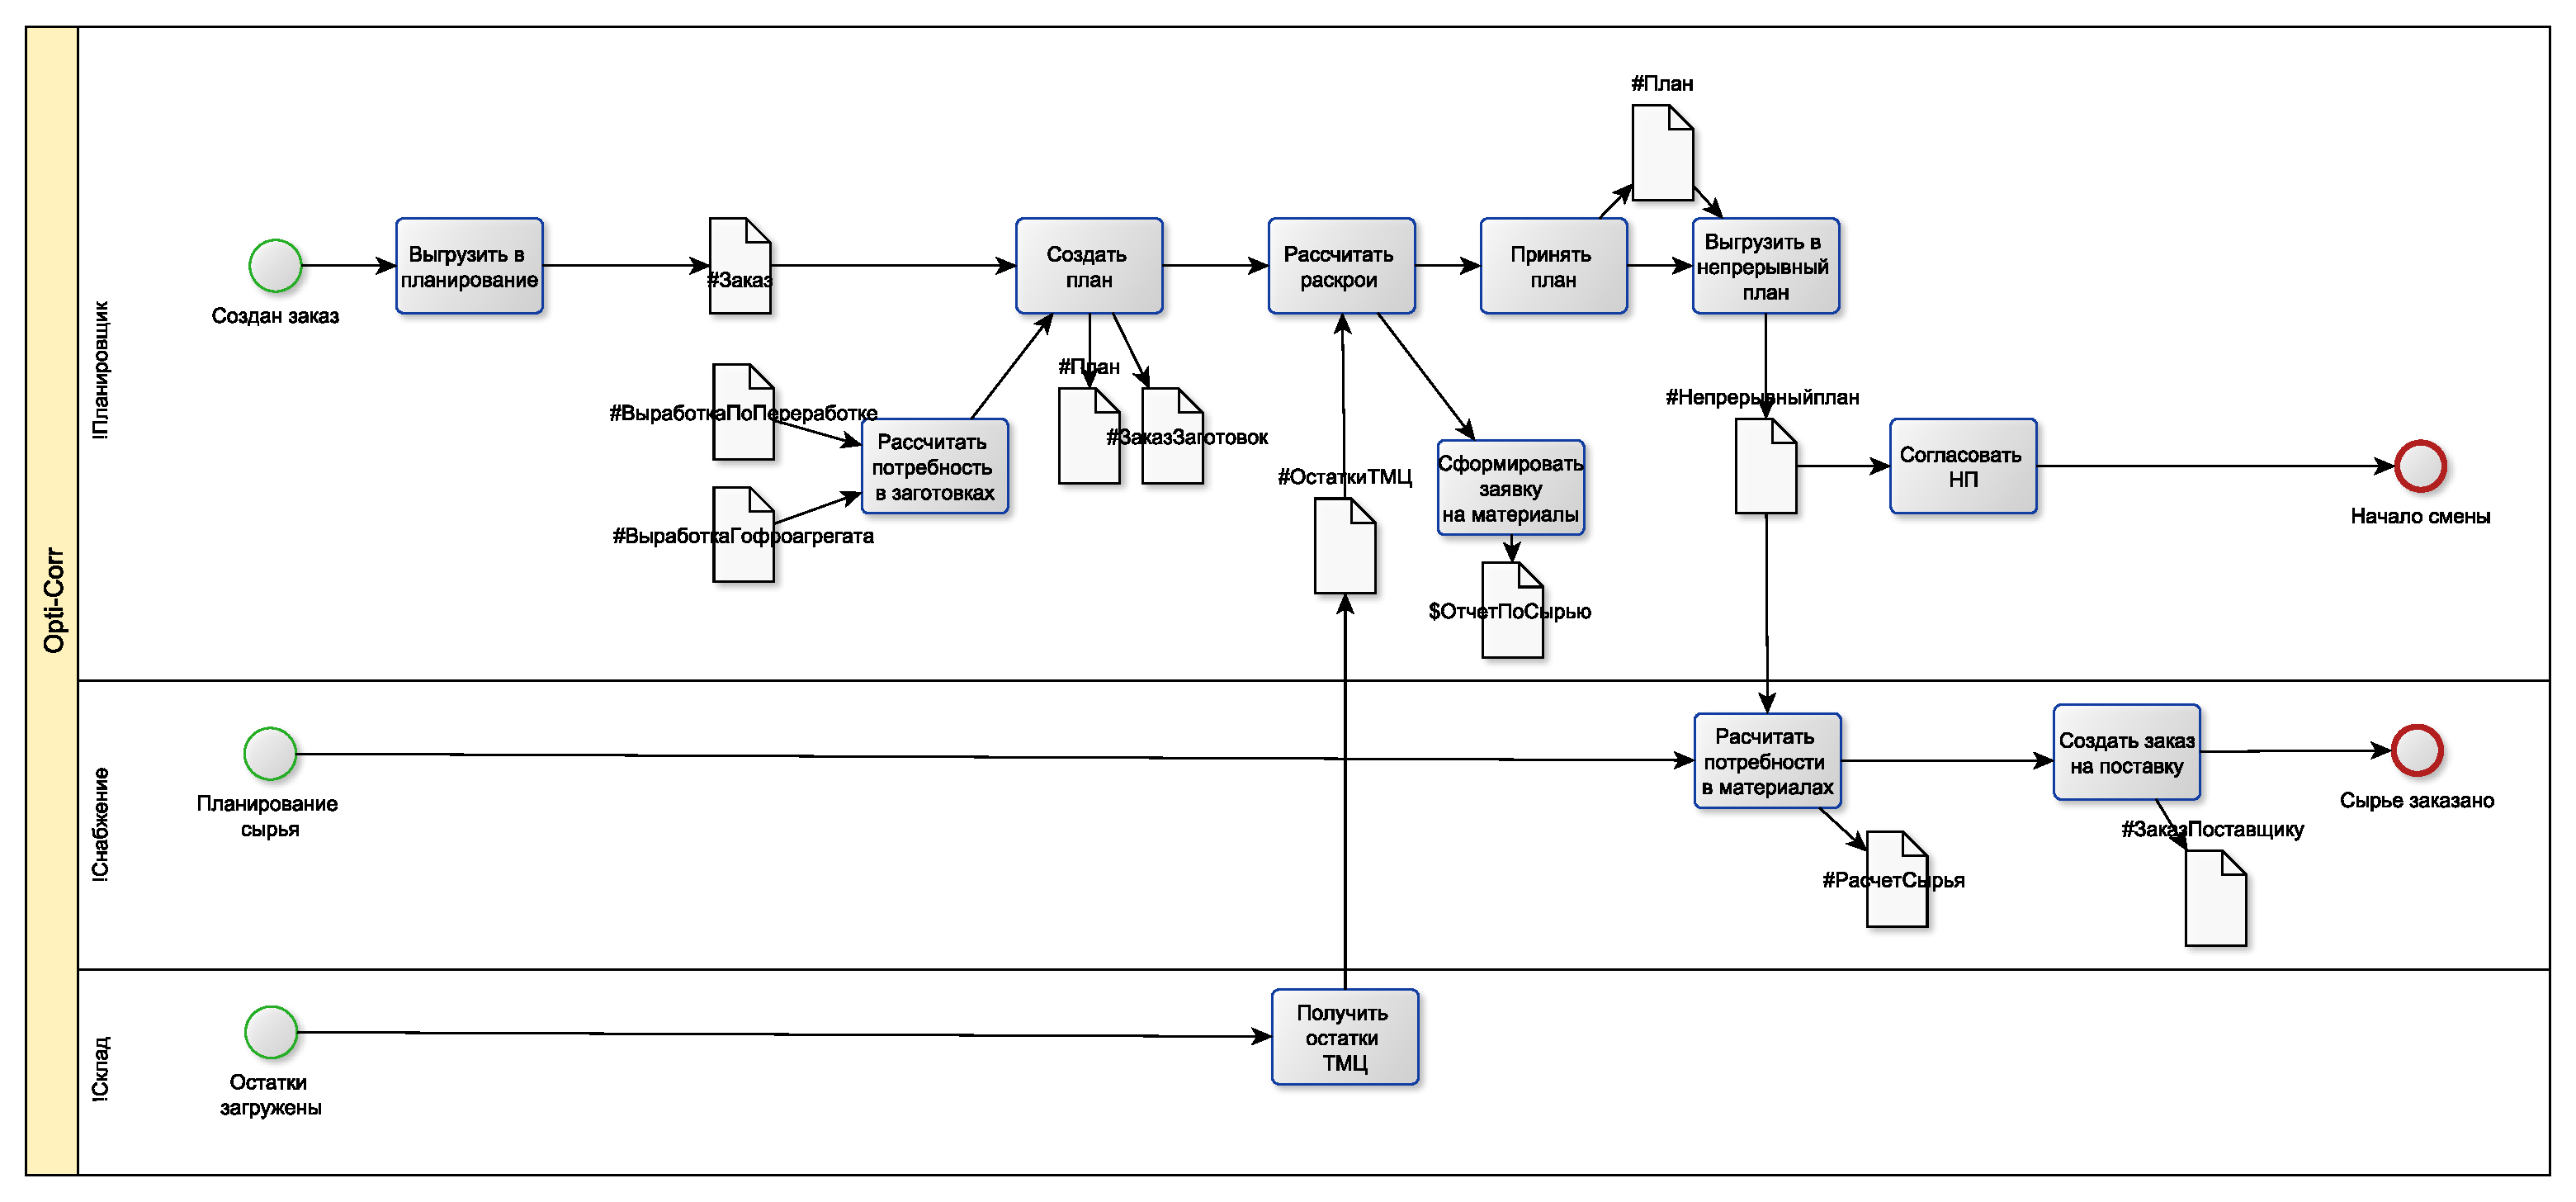
\includegraphics[angle=90, height=0.8\textheight, keepaspectratio]{Pics/3_Планирование и склад материалов.pdf}
\end{center}
  \caption{Процессы 'Предварительное планирование', 'Оперативное планирование'}
  \label{pic:Schema_3}
\end{figure}
\clearpage


Из отдела продаж заказы появляются в СИСТЕМЕ у планировщика с одобренным статусом.

Планировщик выполняет оперативное планирование работы гофроагрегата и линий переработки. По факту планирования работы гофроагрегата Планировщик  в СИСТЕМЕ формирует потребности по материалам, создает при необходимости  документ ''Заказ поставщику''. 
В результате Планировщик формирует оперативный план работы по гофроагрегату и линиям переработки.
План производства доступен на производстве для выполнения.



% По регламенту СИСТЕМА выгружает все складские документы в систему 1С:УНФ.
% %
% %\newpage
% %%
\subsection{Процессы 'Управление производством'}
%
\begin{figure}
\begin{center}
  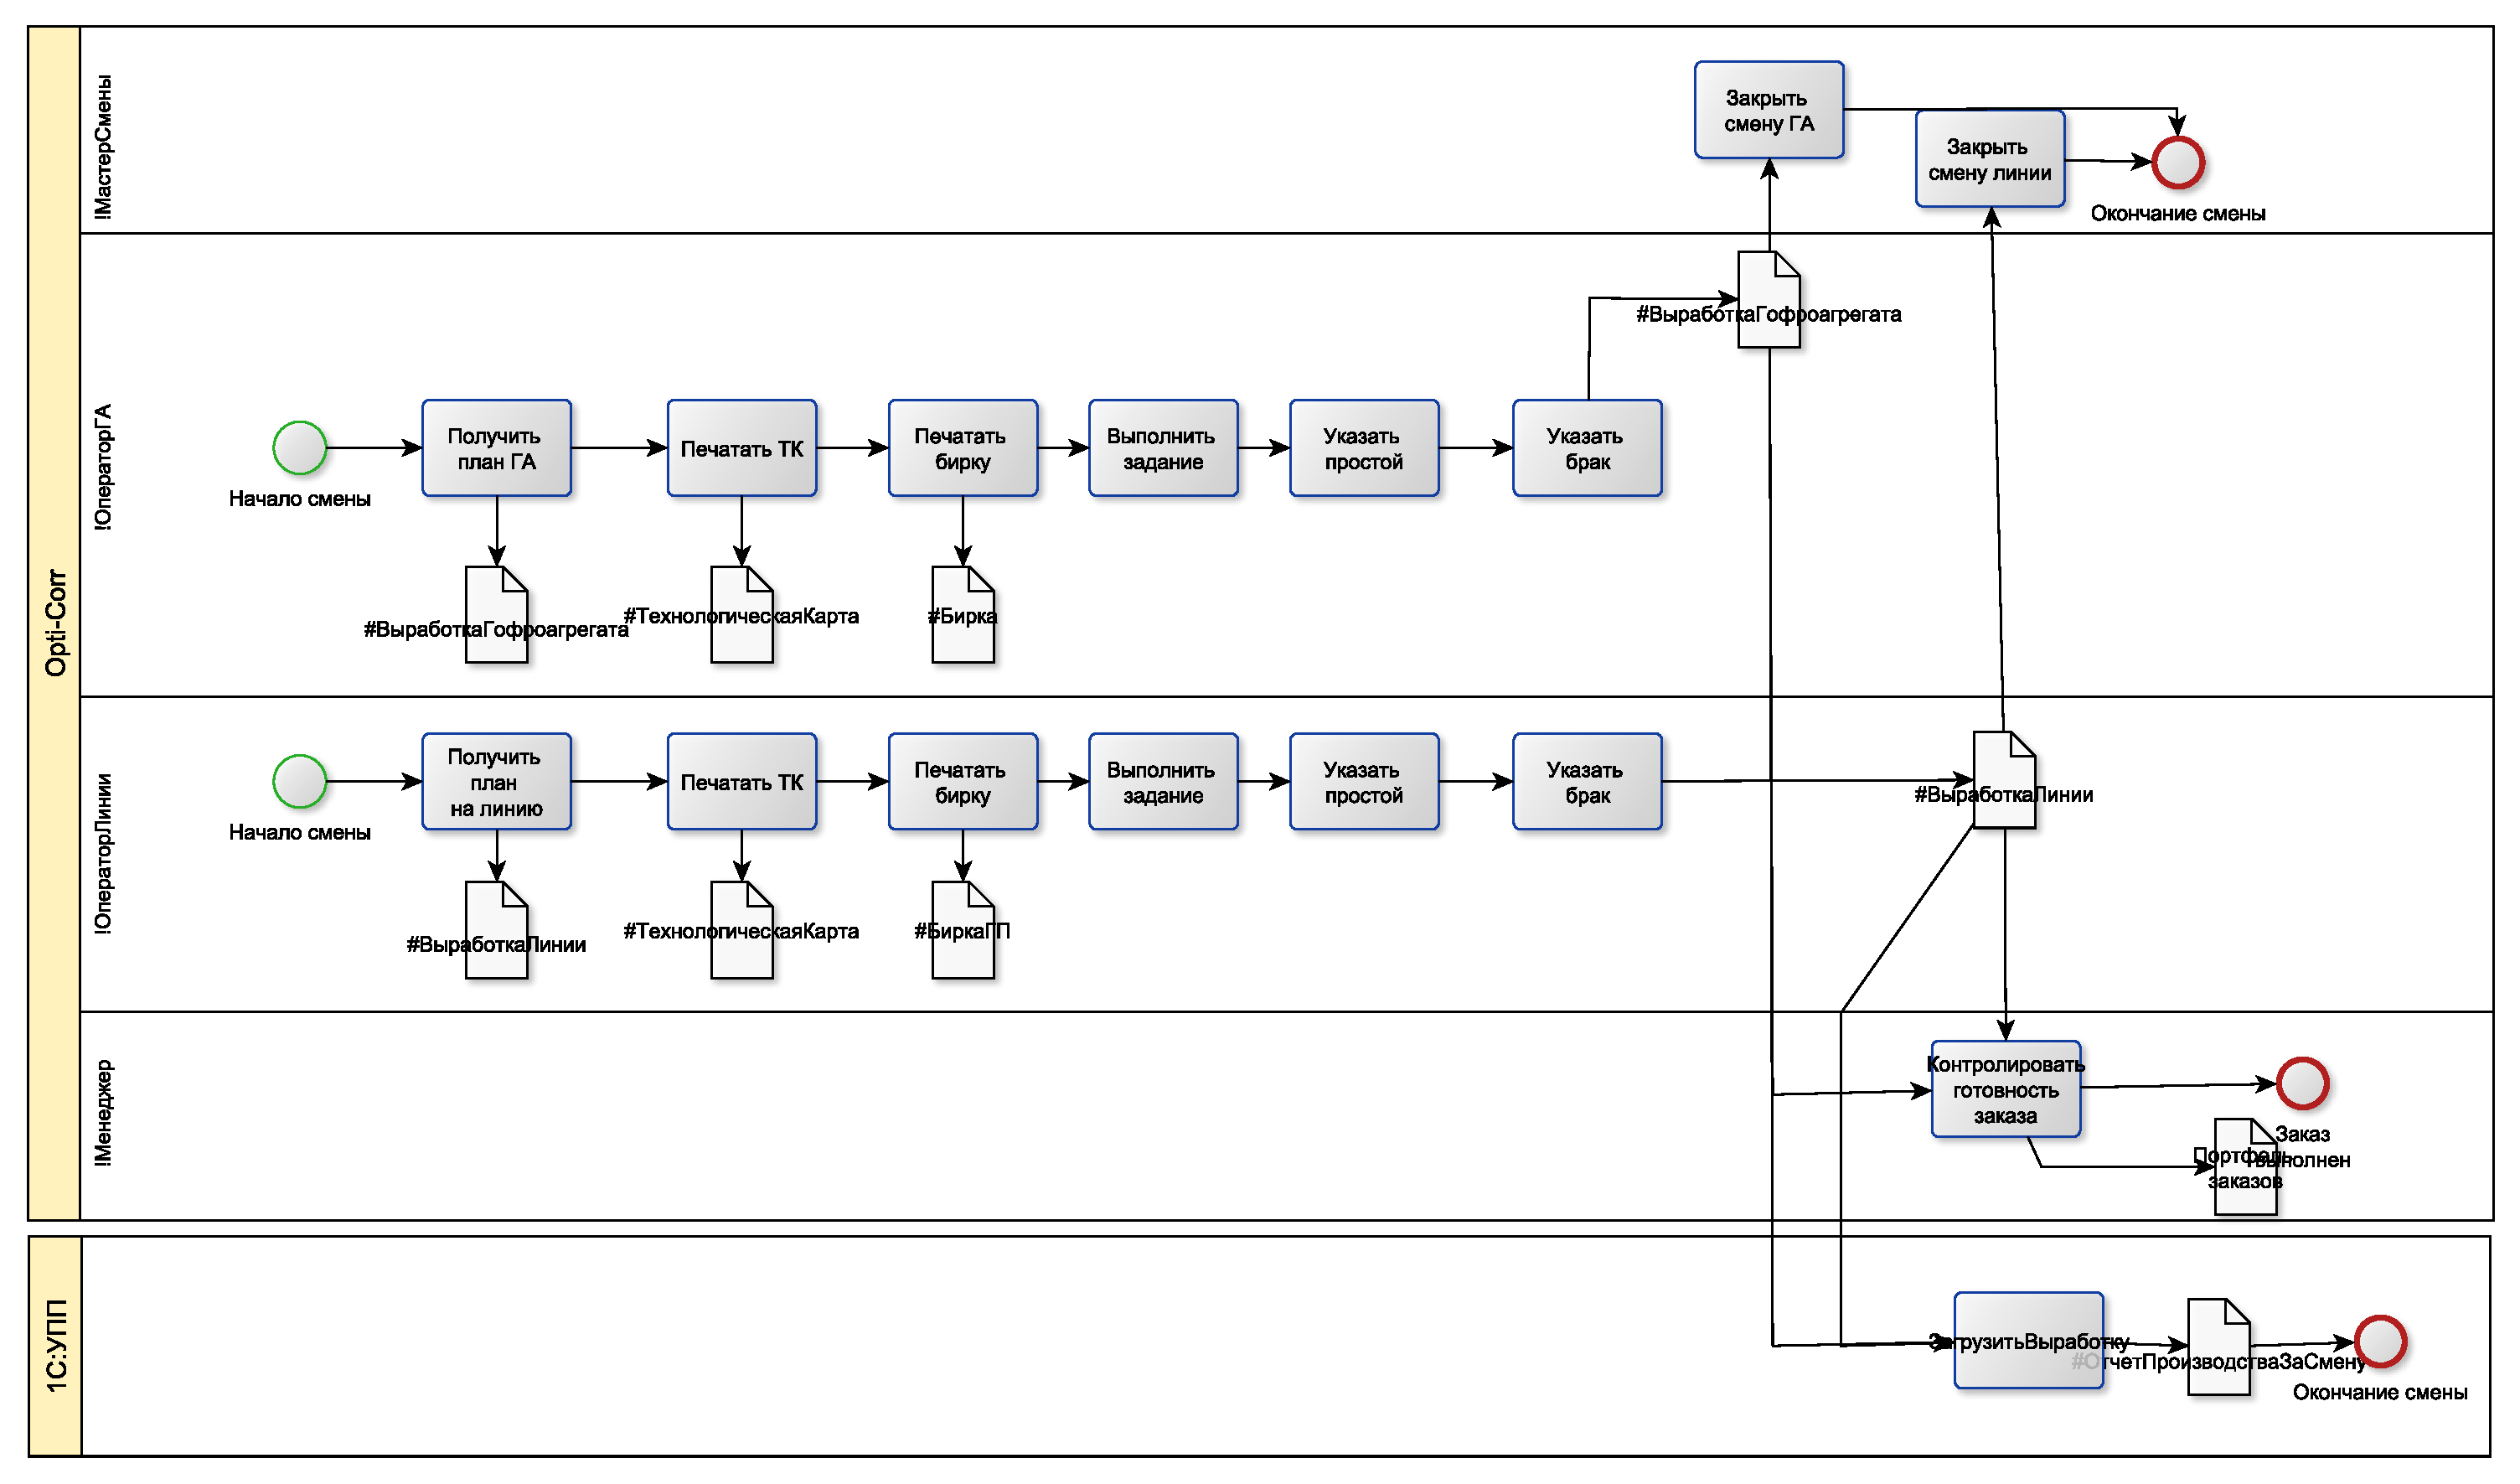
\includegraphics[angle=90, height=0.9\textheight, keepaspectratio]{Pics/4_Выработка.pdf}
\end{center}
  \caption{Процессы 'Управление производством'}
  \label{pic:Schema_4}
\end{figure}
% \clearpage




 Машинист гофроагрегата получает оперативный план производства на своем рабочем месте в СИСТЕМЕ. Машинист гофроагрегата должен в СИСТЕМЕ зафиксировать выработку по гофроагрегату (в документе ''Выработка гофроагрегата''), в т.ч. брак в работе гофроагрегата, простои и остановы.

Машинист на технологической линии получает оперативный план производства линии на своем рабочем месте в СИСТЕМЕ. Машинист технологической линии фиксирует факт выработки по заказу, отклонения, в т.ч. брак при работе линии, простои и остановы.

% Документы по выработке ''Выработка гофроагрегата'', ''Выработка по переработке'' при автоматическом обмене СИСТЕМА выгрузит в документы ''Отчет производства'' в систему 1С:УНФ.

На рабочем месте машиниста гофроагрегата раскрои и план работы будет выгружен в контролер гофроагрегата Fosber и систему Syncro. Обратно автоматически будут загружаться данные по работе гофроагрегата по каждому раскрою. 


\subsection{Процессы 'Планирование отгрузки', 'Управление качеством', 'Управление продажами'}
%
\begin{figure}
\begin{center}
  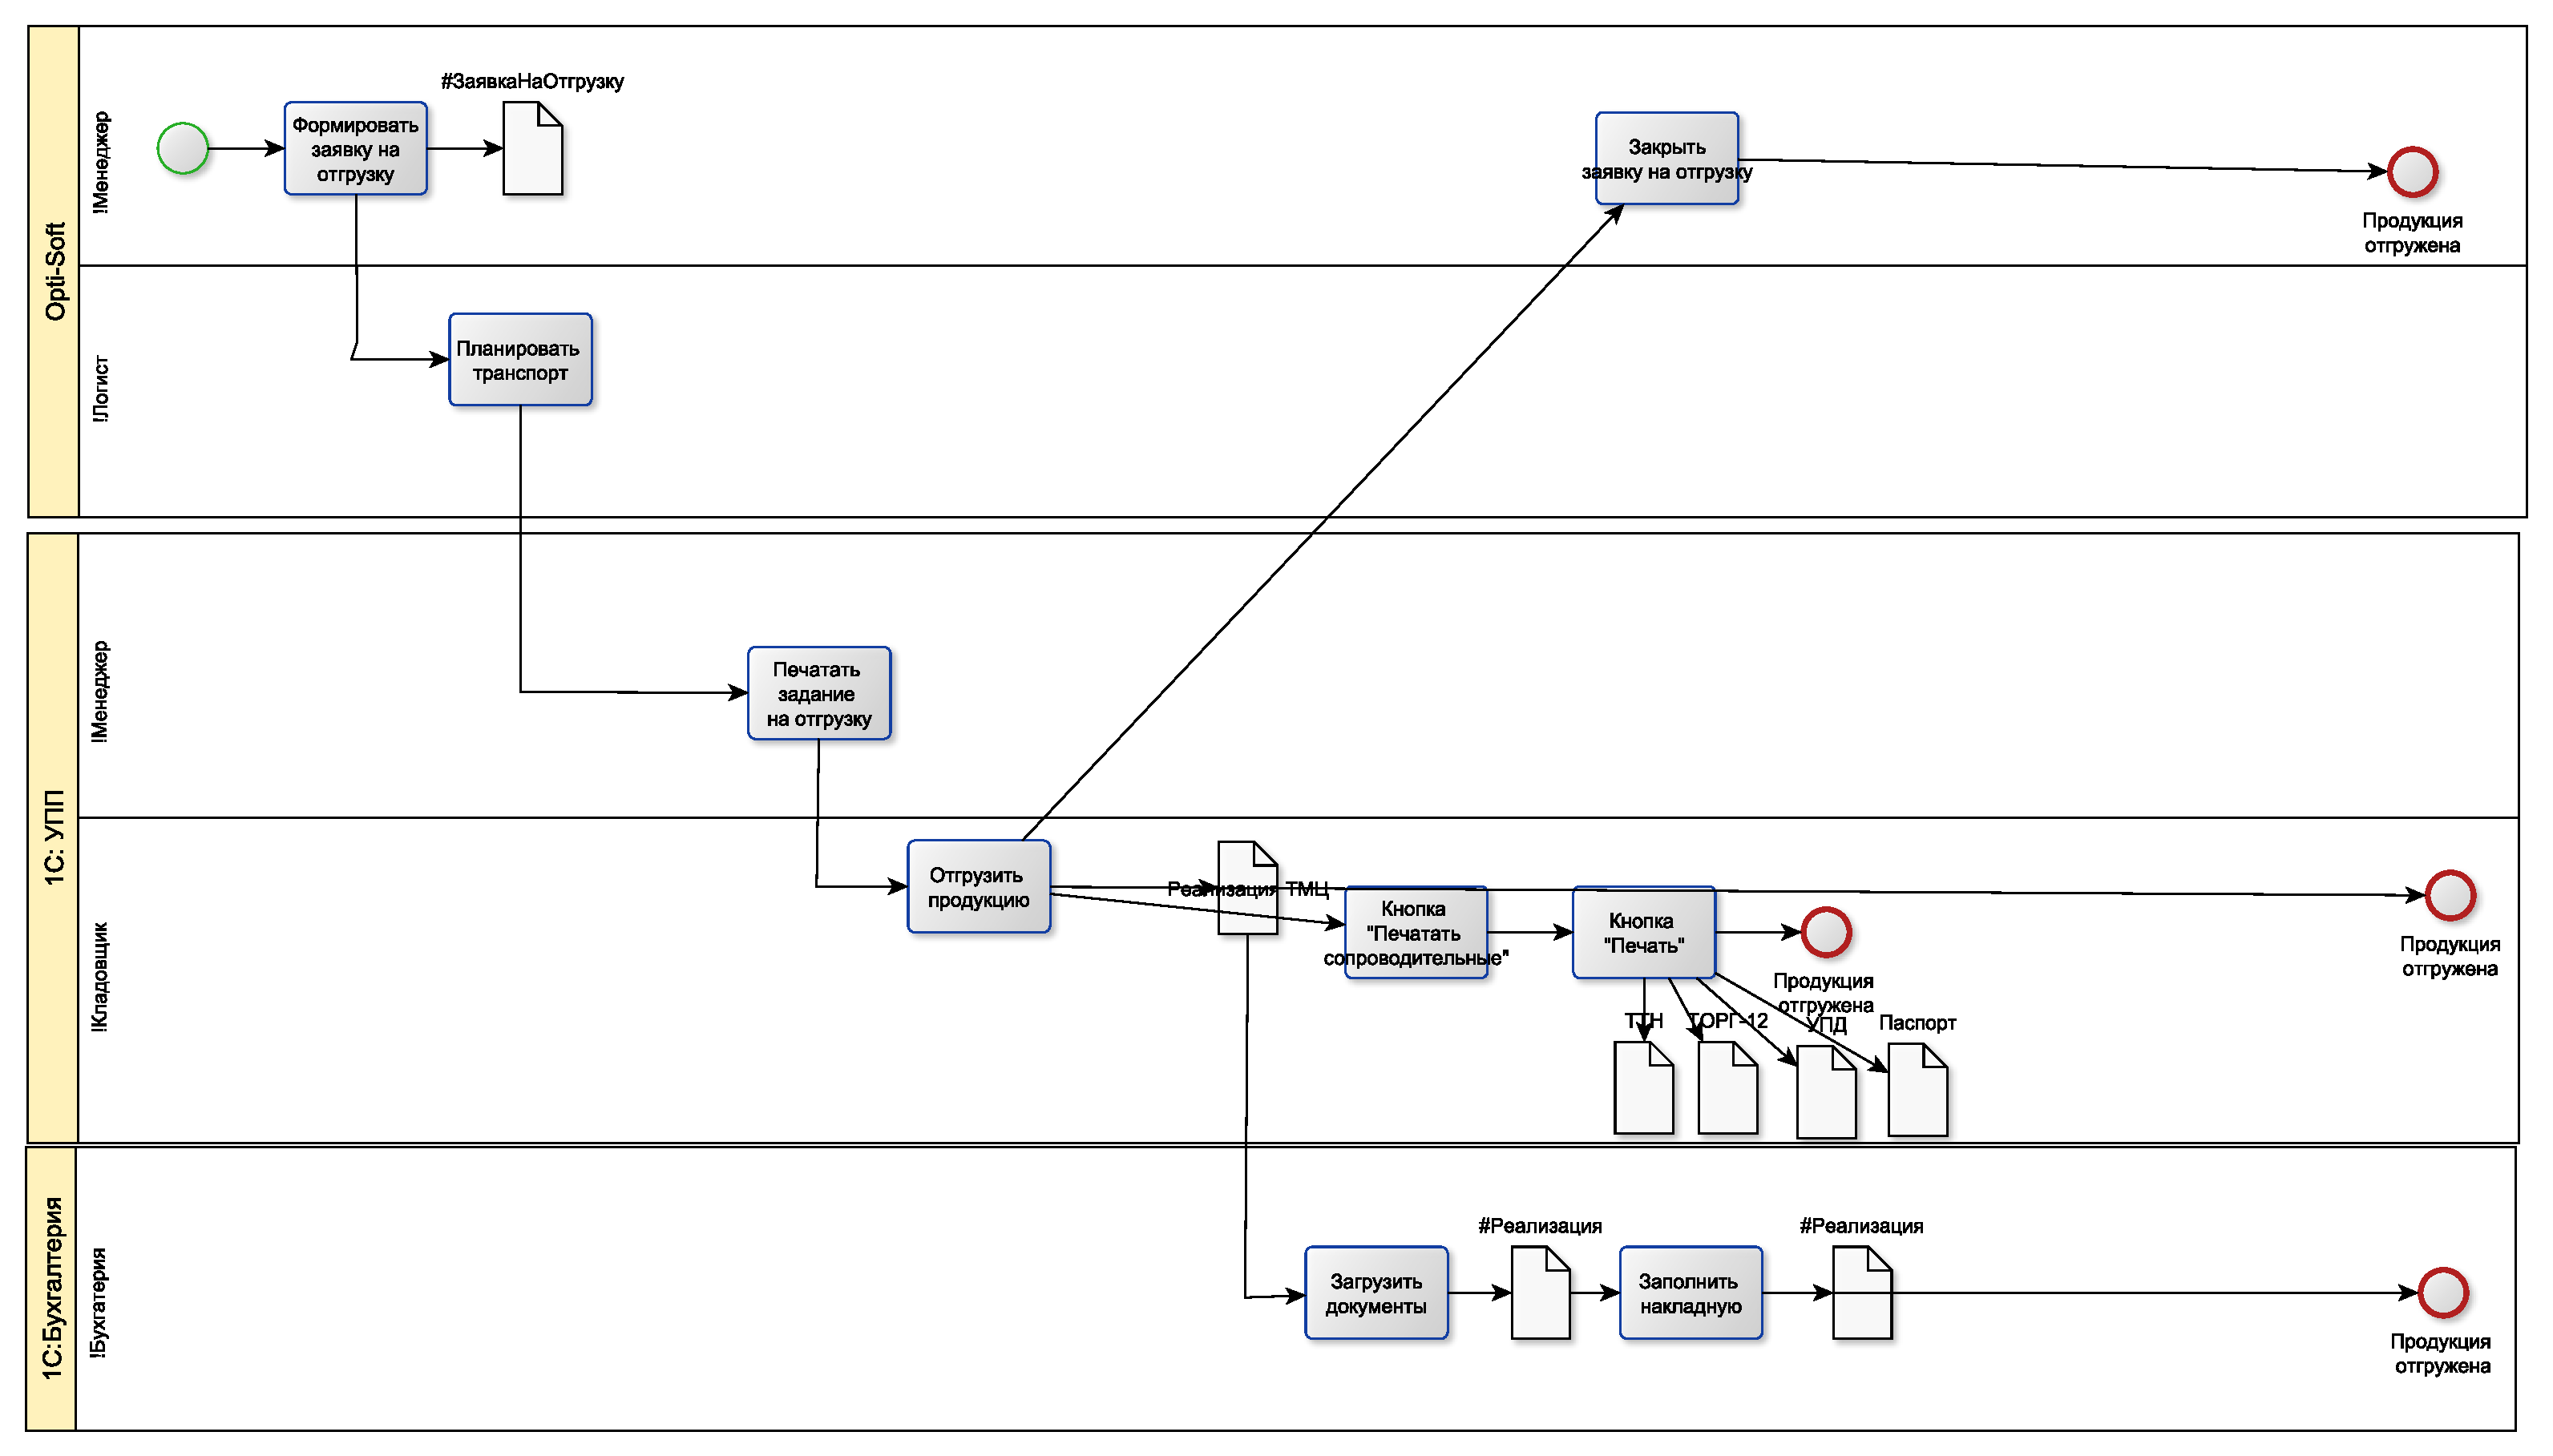
\includegraphics[angle=90, height=0.9\textheight, keepaspectratio]{Pics/5_Отгрузка.pdf}
\end{center}
  \caption{Процессы 'Планирование отгрузки', 'Управление качеством', 'Управление продажами'}
  \label{pic:Schema_5}
\end{figure}
% \clearpage



% Цена продукции по умолчанию будет указана в справочнике ''Номенклатура'' менеджером.


По факту изготовления готовой продукции менеджер будет контролировать в СИСТЕМЕ состояние заказа, его готовность и местоположение.
При готовности заказа менеджер будет создавать в СИСТЕМЕ документ ''Заявка на отгрузку'' либо вручную, либо на основании заявки покупателя.

Заявка будет выгружена в систему 1С:УПП.
Логист отдела продаж в 1С:УПП указывает в документах ''Заявка на отгрузку'' транспорт, который будет подан под погрузку. Логист планирует транспорт под погрузку.

Логист планирует размещение груза в транспортном средстве в 1С:УПП через оптимизатор погрузки.

% Заявка на отгрузку будет автоматически или по запросу выгружена из СИСТЕМЫ в систему СБИС в документ "ЗаявкаНаОтгрузку".

Кладовщик на производстве будет видеть в системе 1С:УПП все распоряжения на отгрузку (Заявка на отгрузку).
При поступлении транспорта кладовщик создает на основании документа ''Распоряжение на отгрузку'' документ ''Реализация ТМЦ''. По факту отгрузки кладовщик корректирует при необходимости факт отгрузки в документе ''Реализация ТМЦ''. 
Кладовщик формирует и печатает сопроводительные документы в системе 1С:УПП: ТН, ТТН.

Бухгалтер формирует и печатает сопроводительные документы в системе 1С:Бухгалтерия: счет-фактура, расходная накладная.

% Документы ''Реализация ТМЦ''  при автоматическом обмене СИСТЕМА выгрузит в документы ''Реализация'' в систему 1С:УНФ.


% %
% %
\subsection{Процессы 'Поступление материалов', 'Списание материалов в производство'}
%
\begin{figure}
\begin{center}
  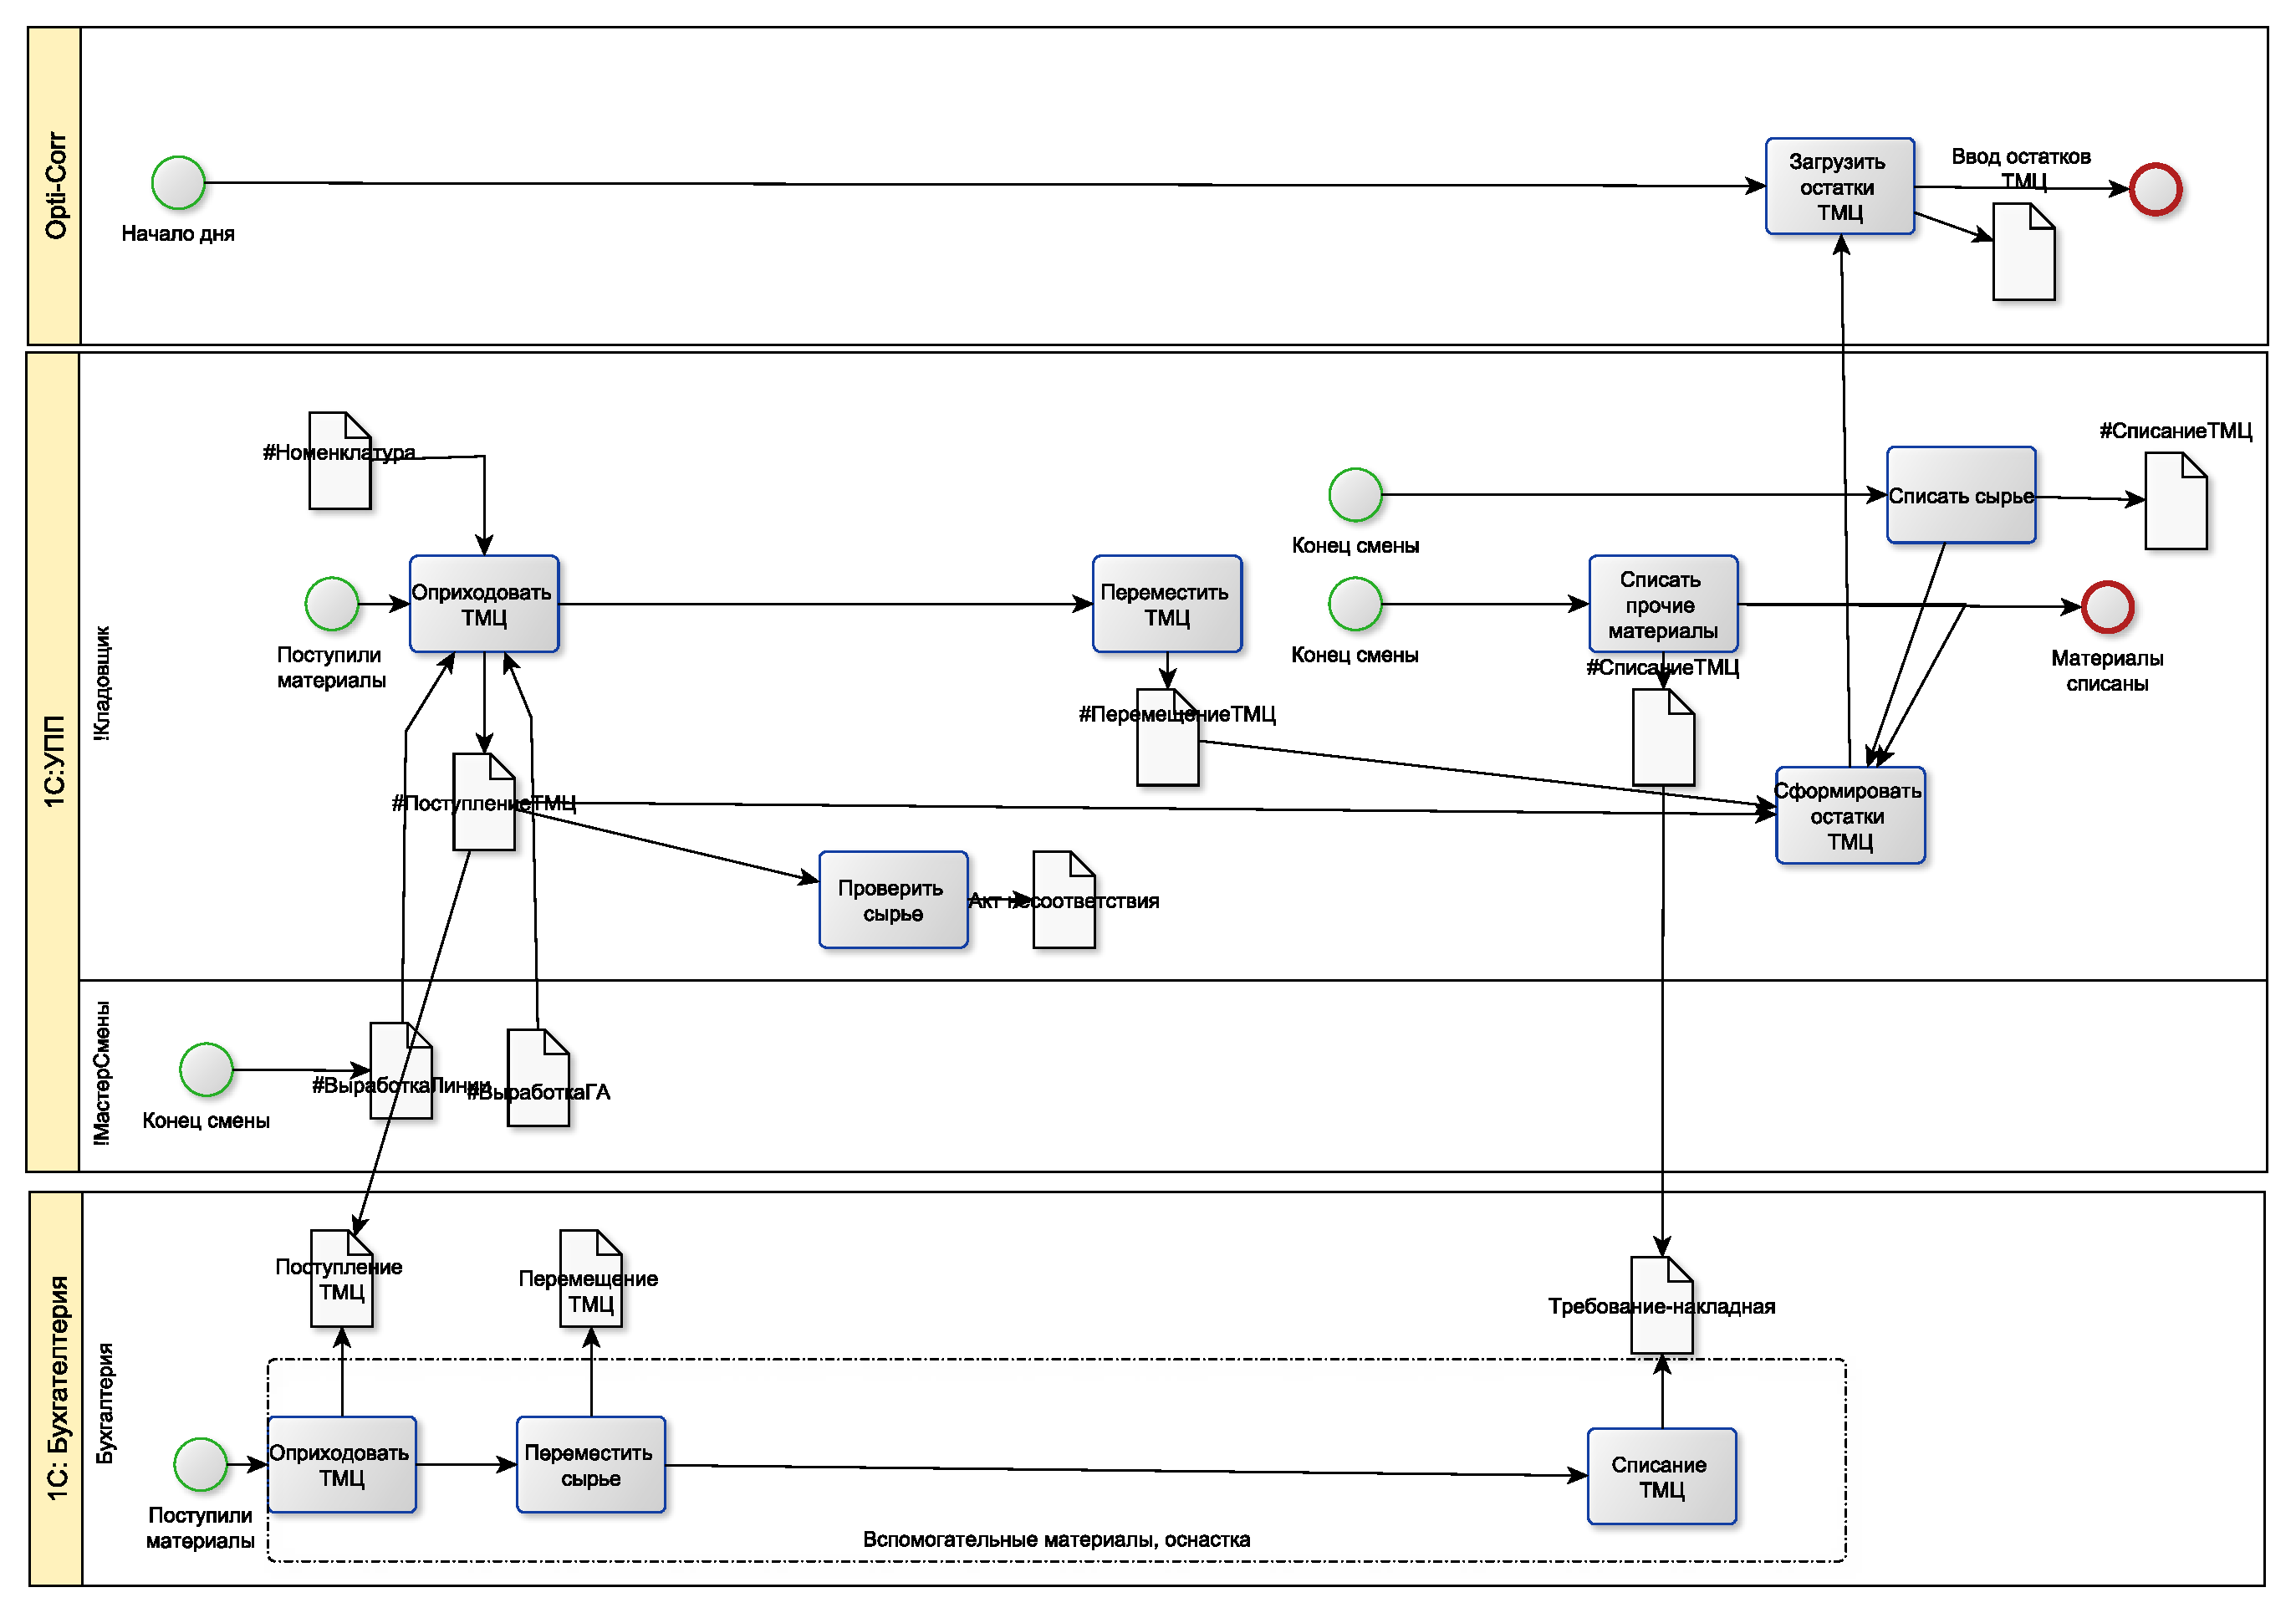
\includegraphics[angle=90, height=0.8\textheight, keepaspectratio]{Pics/6_Учет ТМЦ.pdf}
\end{center}
  \caption{Процессы 'Поступление материалов', 'Списание материалов в производство'}
  \label{pic:Schema_6}
\end{figure}
% \clearpage

Учет материалов остается в системе 1С:УПП как есть.

Остатки по материалам (картон и бумага) загружаются из системы 1С:УПП в СИСТЕМУ каждый день в начало дня. Информация по остаткам материалов используется в СИСТЕМЕ при планировании работы гофроагрегата.

% Материалы (заготовки) будет оприходовать мастер производства в системе Опти-Софт документом ''Поступление ТМЦ''. Рулоны бумаги и картона оприходует кладовщик 
% в системе Опти-Софт документом ''Поступление ТМЦ''.

% При необходимости перемещения рулонов на гофроагрегат кладовщик создает документ ''Перемещение ТМЦ'' в системе Опти-Софт.

% Кладовщик на производстве в СИСТЕМЕ оприходует поступающие материалы и заготовки в СИСТЕМЕ в документе "Поступление ТМЦ". 
% Мастер на производстве фиксирует перемещение ТМЦ документом "Перемещение ТМЦ".

% Операторы на раскатах фиксируют сырье, использованное при производстве гофрокартона, в документе "Сырье для выработки".
% Кладовщик выполняет списание в производство  в СИСТЕМЕ документом ''Списание ТМЦ'' на основании документа "Сырье для выработки".

% Документы автоматически выгружаются в систему 1С:УНФ по регламенту.

%
%
%
%
%
%%
%%\newpage
%%
%%\subsection{Процессы 'Управление и диспетчеризация производства', 'Списание бумаги и картона', 'Управление качеством', 'Учет готовой продукции', 'Планирование отгрузки', 'Отгрузка готовой продукции'}
%%
%%\begin{figure}
%%\begin{center}
%%  \includegraphics[height=0.94\textheight, keepaspectratio]{Pics/Schema_3.jpg}
%%\end{center}
%% % \caption{Процессы 'Управление и диспетчеризация производства', 'Списание бумаги и картона', 'Управление качеством', 'Учет готовой продукции', 'Планирование отгрузки', 'Отгрузка готовой продукции'}
%%  \label{pic:Schema_3}
%%\end{figure}
%%\clearpage
%